\documentclass{article}
\usepackage{graphicx}
\usepackage[normalem]{ulem}
\usepackage[margin=1.5cm]{geometry}
\usepackage{amsmath}

\begin{document}

\title{Laboratory on Net Force: Force Tables}
\author{Prof. Jordan C. Hanson}

\maketitle

\begin{figure}[ht]
\centering
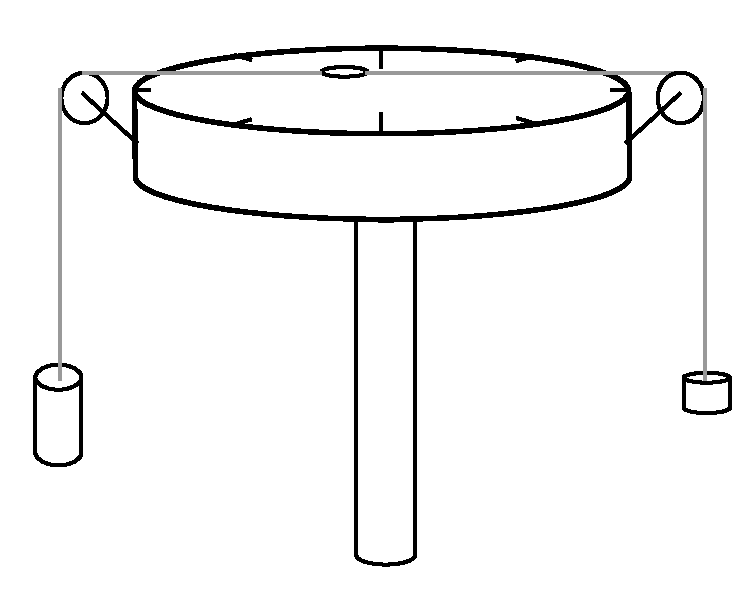
\includegraphics[width=0.25\textwidth]{figures/Table.pdf}
\caption{\label{fig:table} The force table setup includes a wheel with angles, strings and pulleys, and a central ring.}
\end{figure}

\section{Force Table Lab Setup}

Obtain a set of weights, and a force-table, with ring and pulley system.  Using knowledge of vectors, arrange weights on the pulleys such that the ring remains stationary in the center.  Double one of the weights, and find the angles the strings must make to keep the ring stationary in the center.  Define the force vectors as vectors with magnitudes equal to the masses of the weights, in the directions of the strings.  Do the vectors add to zero?
\noindent
\\ \\
Now remove the weights from the three strings.  Make the angle between two of the strings 60 degrees.  Choose two different weights, $m_1$ and $m_2$.  Set $m_1$ on 0 degrees, and set $m_2$ on 60 degrees.  We will determine the weight $m_3$ that cancels these tensions to keep the ring stationary if hung at the correct angle.  We will test the hypothesis by hanging the weights and observing if the ring moves.

\section{Details of the Measurement}

\begin{enumerate}
\item The \textit{weight force} causing the tension by a mass $m$ on the ring is $\vec{w} = m g \hat{x}$, where $\hat{x}$ represents the direction the string is pulling, $g$ is acceleration due to gravity, and $m$ is the mass.  Let $m_1$ and $m_2$ be the two masses you have chosen to be 60 degrees apart.  Make the string attached to $m_1$ align with 0 degrees on the table, and $m_2$ align with 60 degrees on the table.
\item Treating the tension $\vec{T}_1$ (with $m_1$) and the tension $\vec{T}_2$ (with $m_2$) as vectors, break them into components:
\\
\underline{$T_{1,x}=$ \hspace{1cm} (N)} \hspace{0.5cm} \underline{$T_{1,y}=$ \hspace{1cm} (N)} \hspace{0.5cm} \underline{$T_{2,x}=$ \hspace{1cm} (N)} \hspace{0.5cm} \underline{$T_{2,y}=$ \hspace{1cm} (N)}
\item Determine $\vec{T}_3$ such that $\vec{F}_{\rm Net} = 0$:
\begin{table}[hb]
\centering
\begin{tabular}{| c | c | c |}
\hline
Vector & x-component (N) & y-component (N) \\ \hline
$\vec{T}_1$ & & \\ \hline
$\vec{T}_2$ & & \\ \hline
$\vec{T}_3$ & & \\ \hline
$\vec{F}_{\rm Net}$ & & \\ \hline
\end{tabular}
\caption{\label{tab:data} Break the vectors into components here.}
\end{table}
\item Knowing that $|\vec{T}_3| = m_3 g$, solve for $m_3$.  Knowing the components of $\vec{T}_3$, solve for the angle it makes with the x-axis (0 degrees).  Arrange $\vec{T}_3$ on the table.  \textbf{Is the ring stationary?}
\end{enumerate}

\end{document}
